\documentclass[a4paper,9pt]{article}
\usepackage[utf8]{inputenc}
\usepackage[left=1cm,top=1.5cm,right=1cm,bottom=1.5cm]{geometry}
\usepackage{multicol}
\usepackage{graphicx}
\usepackage[parfill]{parskip}
\usepackage{utopia}
\usepackage{fancyhdr}
\pagestyle{fancy}
\fancyhf{}
\rhead{CC-NC-SA}
\lhead{BMS Abschlussprüfung Physik}
\rfoot{\thepage}
\lfoot{Juni 2017}

\begin{document}
\begin{multicols}{4}
	\textbf{Schiefe Ebene} \\
	\includegraphics[width=4cm]{gr1}
	

\textbf{Kraft (allgemein)} \\
	\(F = m * a\)
	

\textbf{Auf horizontaler Ebene} \\
	\(F_N = F_G = g * m\)
	

\textbf{Hangantriebskraft} \\
	\(F_{G,P} = F_G * sin(\alpha)\)
	

\textbf{Normalkraft} \\
	\(F_{G,S} = F_N = \cos\alpha*F_G\)
	

\textbf{Reibungskraft} \\
	\(F_R = F_N * \mu\)
	

\textbf{Steigung \% - Grad} \\
	\(\alpha = \arctan(m) \)
	

\textbf{Ab wann rutscht der Körper von selbst?} \\
	\(\alpha = \arctan(\mu)\)
	
	 (Bsp: \(\mu = 0.51, \alpha = \arctan(\mu) = 27^\circ\))
	
	
	
	
	

\textbf{\textit{Kreisbewegung}} \\
	

\textbf{Gleichförmige Kreisbewegung} \\
	\includegraphics[width=3cm]{gr2.png}
	$ T=\Delta t $
	
	$ v=\frac{\Delta s}{\Delta t} $
	
	

\textbf{Drehfrequenz} \\
	
	$ f = \frac{n}{t} $ ( $n$ = Umdrehungen)
	
	$ [f] = \frac{1Hz}{1s} $
	
	$ v = 2\pi * r * f $
	
	

\textbf{Kreisfrequenz o. Winkelgeschw.}\\
	
	$ w = \frac{2\pi}{T} $ auch $ w = 2\pi f $
	
	

\textbf{Zentripetalbeschleunigung / Radialbeschleunigung $ \vec{a_z} $ }\\
	\includegraphics[width=3cm]{gr3}
	
	$ \vec{\Delta v} = \vec{v_2} - \vec{v_1} $
	
	$ a_z = \frac{\Delta v}{\Delta t} $ u. $ a_z = \frac{v^2}{r} $ u. $ a_z = r*w^2 $
	
	

\textbf{Klötze auf Drehscheibe}\\
	
	\includegraphics[width=3cm]{gr4}
	
	Klotz bleibt auf Scheibe solange $ F_Z \le F_R $ also $ \frac{m * v^2}{r} \le \mu_H * , * g $
	
	$ v \le \sqrt{\mu_H * r * g} $
	
	$ m * w^2 * r \le \mu_H * m * g \Rightarrow w \sqrt{\frac{\mu_H * r *g}{r}} $
	
	

\textbf{Überhöhte Kurven ohne Reibung}\\
	\includegraphics[width=4cm]{gr5}
	
	$ \vec{F_Z}  = \vec{F_G} + \vec{F_N} $
	
	$ \tan{\alpha} = \frac{F_Z}{F_G} = \frac{m*\frac{v^2}{r}}{m*g} $ also $ \alpha = arctan(\frac{v^2}{r} *g) $  
	
	

\textbf{Bsp. Schaukel}\\
	
	\includegraphics[width=3cm]{gr6}
	
	$ F_{Res} = F_Z = F_N - F_G  $
	
	also $ F_N - F_G + F_Z = m * g + m\frac{v^2}{z} $
	
	

\textbf{Looping}\\
	
	\includegraphics[width=3cm]{gr7}
	
	Funktioniert wenn $ F_Z > g $ also $ v \ge \sqrt{r * g} $
	
	$ F_{res} = F_Z $ und $ F_{res} = F_N + F_G $
	
	also $ F_N = F_Z - F_G = m(\frac{v^2}{r}*g) $
	
	

\textbf{\textit{Gravitation}}\\
	

\textbf{Konstanten}\\
	

\textbf{G} Gravitationskonstante:\\
	\(G=6.67408*10^{-11}\frac{m^3}{kg*s^2} \)
	

\textbf{Kraft}
	\(F=G\frac{m_1 m_2}{r^2} \)\\
	\includegraphics[width=3cm]{radius}\\
	

\textbf{Daraus ableitend:}\\
	\(a_1 = \frac{F_1}{m_1}=G\frac{m_2}{r^2} \)\\
	

\textbf{und}\\
	\(a_1 + a_2 = G\frac{m_1 + m_2}{r^2}\)\\
	

\textbf{\textit{Luftwiderstand}}\\
	

\textbf{Konstanten \& andere Werte}\\
	\(\rho\): Dichte\\
	\(c_w\): Luftwiderstandskoeffizient
	

\textbf{Basisformel}\\
	\( F_w = \frac{1}{2} c_w A  \rho v^2 \)
	

\textbf{Maximalgeschwindigkeit}\\
	\(v_{max} = \sqrt{\frac{2mg}{Ac_w\rho}} \)\\
	In diesem Fall ist \(F_w = F_G\)
	
	

\textbf{Masseinheiten}\\
	\textit{jeweils nach SI}\\
	\begin{tabular}{|l|l|l|}
		\hline
		

\textbf{Name} & 

\textbf{Bez.} & 

\textbf{SI} \\\hline
		Leistung & \(P\) & \(W\)\\\hline
		Energie & \(E\) & \(J\) \\\hline
		Kraft & \(F\) & \(N\)\\\hline
	\end{tabular}
	
	\textit{Andere Einheiten}\\
	\(1 PS = 735,49875 W\)\\
	
	
	

\textbf{Leistung}\\
	

\textbf{Grundformel}\\
	\(P = \frac{\Delta E}{\Delta t} = \frac{\Delta W}{\Delta t} \)\\
	und\\
	\(P = \vec{F} * \vec{v}\)
	
	

\textbf{Wirkungsgrad}\\
	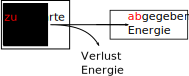
\includegraphics[width=4cm]{wirkungsgrad}\\
	

\textbf{Grundformel}\\
	\(\eta = \frac{{\Delta {E_{ab}}}}{{\Delta {E_{zu}}}} = \frac{{{P_{ab}} \cdot \Delta t}}{{{P_{zu}} \cdot \Delta t}} \Rightarrow \eta = \frac{{{P_{ab}}}}{{{P_{zu}}}}\)
	\\
	Regel: \(\eta \leq 1\)
	

\textbf{\textit{Energie}}\\
	

\textbf{Bewegungsenergie}\\
	
	\(E_{kin} = \frac{1}{2} mv^2\)
	
	

\textbf{Potenzielle Energie}
	
	\(E_{pot} = m * g * h\)\\
	Beispiel: Im freien Fall ist \(E_{pot} = E_{kin}\)\\
	
	
	

\textbf{\textit{Energieerhaltungssatz}}\\
	

\textbf{Grundformel}\\
	\(E = E_1 + E_2 + E_3 + \dots + E_n\) und immer \(\Delta E = 0\)\\
	
	

\textbf{\textit{Hydrostatik}}\\
	

\textbf{Grundformel}\\
	\begin{itemize}
		\item \(g\): Erdbeschleunigung
		\item \(\rho_{Fluessigkeit}\): Dichte der Flüssigkeit in \(kg\)
		\item \(h\): Höhe der Flüssigkeitssäule in \(m\)
	\end{itemize}
	\(\rho = \rho_{Fluessigkeit} * g * h\)\\
	Abstrakt:\\
	\(Druck = \frac{Kraft}{Flaeche}\); \(\rho = \frac{F}{A}\) \\
	\includegraphics[width=4cm]{hydrostatik}
	\textit{Der hydrostatische Druck am Boden ist trotz unterschiedlicher Füllmengen in allen drei Gefäßen gleich groß.}
	
	  

\textbf{Wärmelehre}\\
	  $ 0 K = - 273.15 C^\circ $ (allgemein $ 0 K = 273^\circ C $)
	  
	  

\textbf{\textit{Wärme-ausdehnung}}\\
	  

\textbf{Linear}\\
	  
	  $ \Delta l = \alpha * l_0 * \Delta \vartheta $ also
	  
	  $ l = l_0 * (1 + \alpha * \Delta \vartheta) $
	  
	  $ \alpha = \frac{\Delta l}{l_0 * \Delta \vartheta} $
	  
	  

\textbf{Volumen}\\
	  
	  

\textbf{Initialzustand:}\\
	  
	  $ V_0 = l_0 * b_0 * h_0 $
	  
	  \textit{In erwärmten Zustand}\\
	  
	  $ V = l * b * h = l_0 (1 + \alpha * \Delta \vartheta) * b_0 (1 + \alpha * \Delta \vartheta) * h_0 (1 + \alpha * \Delta \vartheta) $\\
	  
	  

\textbf{Vereinfacht:}\\
	  
	  $ V \approx V_0 (1 + 3 * \alpha * \Delta \vartheta) $\\
	  
	  $ \gamma = 3 * \alpha $ \\
	  
	  \textit{Volumenzunahme $\Delta V$:}\\
	  $ \Delta V = V_0 * \gamma  * \Delta \vartheta $ \\
	  
	  

\textbf{Wärmeenergie}\\
	  
	  

\textbf{Wärmeenergie}: $[Q] = Joule (J) = Newtonmeter (Nm)$\\
	  

\textbf{Wärmekapazität}: $ [c] = \frac{kJ}{kg K}$\\
	  
	  

\textbf{Beispiele für $ c $}\\ 
	  \begin{tabular}{ll}
	  	Wasser & 4.19 \\
	  	Alkohol & 2.43 \\
	  	Wasserstoff & 14.3
	  \end{tabular}\\
	  
	  

\textbf{Berechnung:}\\
	  $ \Delta Q = c * m * \Delta \vartheta $
	  
	  

\textbf{Wärmeinhalt}\\
	  $ Q = m * c * \vartheta $
	  

\textbf{Wärmekapazität $[C]$}\\
	  
	  $ [C] = \frac{J}{K} $
	  
	  

\textbf{Berechnung}\\
	  $ C = \frac{\Delta Q}{\Delta \vartheta} $\\
	  
	  Oder \\
	  
	  $ C = m * c $
	  
	  

\textbf{Wärmemischung}\\
	  
	  $ |\Delta Q_{ab}| = | \Delta Q_{auf} | $\\
	  oder\\
	  $c_1 * m_1  * (\vartheta_1 - \vartheta_m) = c_2 * m_2 * (\vartheta_m - \vartheta_2) $\\
	  (Wenn abs wert, ist reihenfolge v. $ \vartheta_{1,2}$ und $ \vartheta_m $ egal)
	  
	  

\textbf{Verbrennungs-energie}\\
	  
	  \textit{Heizwert}: $ H = \frac{Q}{m}; [H] = \frac{J}{kg} $
	  

\textbf{Aggregats-zustände}\\
	  
	  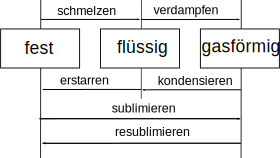
\includegraphics[width=2in]{agregat}
	  
	  

\textbf{Schmelzwärme}\\
	  
	  $ L_F = \frac{Q_s}{m} $
	  
	  

\textbf{Verdampfungs-wärme}\\
	  
	  $ Q_v = \frac{Q_v}{m} $
          
	
	
\end{multicols}	
\end{document}